%% ============================================================================
%% Capítulo 7 — Destilação Distribucional de Foundation Models
%%
%% Fontes (auditadas; nenhum número sem origem em artefato versionado):
%%   - latex/ai2/main.tex .................. formulação final auditada do AI-2
%%     (método, setup, resultados 5.1-5.5, discussão, limitações) — prevalece
%%     sobre o rascunho dissertation/cap7-destilacao.md em caso de divergência
%%   - docs/desenho-experimental-destilacao.md ... pré-registro original
%%     (15-18/07/2026) de H1-H3, protocolo e critérios de decisão
%%   - docs/desenho-melhorias-finais.md .......... pré-registro do E1
%%     (05/10/2026, antes da execução) + adendo de vereditos pós-execução
%%   - docs/memo-novidade-destilacao.md .......... checagens de novidade
%%     datadas (15/07, 20/07 e 04/10/2026)
%%   - results/distillation/baselines_analysis.csv ... dados do E1; 17/20,
%%     p=0,0013 (sinal) / p=0,0008 (Wilcoxon), reveses e latências
%%     recomputados do CSV (pandas/scipy) em 05/10/2026
%%   - results/distillation/{distill,extension,pareto,ablation_*,
%%     mlp_students,classical_baselines}.csv; paper_retention.csv
%%
%% Figuras (copiadas para dissertacao/images/ em 05/10/2026):
%%   - images/pareto_distill_en.pdf ....... de results/figures/pareto_distill_en.pdf
%%   - images/calibration_distill_en.pdf .. de results/figures/calibration_distill_en.pdf
%%   - diagrama do pipeline: TikZ inline (portado de latex/ai2/main.tex,
%%     fig:pipeline, rótulos traduzidos)
%% ============================================================================

\chapter{Destilação Distribucional de Foundation Models}
\label{chap:destilacao}

O Capítulo~\ref{chap:framework} deixou um único obstáculo entre o
praticante e a política regret-ótima ``\emph{foundation model}
primeiro'': o custo de servir. Este capítulo tem como objetivo atacar
esse obstáculo por destilação de conhecimento, com um recorte
verificado como inédito --- a \emph{regressão distribucional}:
transferir não a média, mas a distribuição preditiva completa do
\emph{professor} (\emph{teacher}) para um aluno de microssegundos.
Além disso, sob desenho registrado em duas etapas e auditado com a
correção sequencial correspondente (Seção~\ref{sec:destil-desenho}),
em 20 conjuntos de dados,
confronta-se a destilação com as alternativas de engenharia de
\emph{serving} e com \emph{baselines} distribucionais clássicos, e os
sucessos e fracassos convertem-se na regra de decisão prática que
encerra o capítulo.

\section{Motivação e checagem de novidade}
\label{sec:destil-motivacao}

\subsection{O preço do novo líder}
\label{sec:destil-preco}

O Capítulo~\ref{chap:benchmark} estabeleceu que a geração 2026 de
\emph{foundation models} tabulares quebra o empate histórico de acurácia; o
Capítulo~\ref{chap:framework}, que a política fixa ``\emph{foundation model}
primeiro'' é regret-ótima na métrica primária, com \emph{regret} mediano
0,000 sob validação \emph{leave-one-dataset-out}. O único obstáculo a
essa política é o custo de servir --- e ele não é um detalhe de
implementação, mas uma propriedade constitutiva do paradigma: modelos
de aprendizado em contexto (\emph{in-context learning}) carregam o
conjunto de treino como contexto em cada predição. Sob protocolo
padronizado no conjunto \texttt{adult}, medimos 7.416~\us/linha para o
TabPFN e 43.262~\us/linha para o TabFM, contra 0,33~\us/linha do
XGBoost ajustado --- fatores de aproximadamente $22.000\times$ e
$131.000\times$, respectivamente. A Seção~\ref{sec:regret-ponderado}
mostrou, ademais, que basta deslocar 10--20\% do peso da acurácia para
a latência para que a recomendação se inverta: remover esse obstáculo
não é otimização marginal, é a condição para que a política
regret-ótima seja utilizável em produção.

A ferramenta clássica para esse ataque é a \textbf{destilação de
conhecimento} \citep{bucila2006,hinton2015}: treinar um aluno rápido
nas saídas de um professor caro. Para \emph{foundation models} tabulares, a
literatura a estabeleceu em \emph{classificação}
\citep{pocketfm2026}; a questão deste capítulo é o que ela pode e não
pode transferir em \emph{regressão} --- em particular na regressão
distribucional, em que a saída do professor não é um número, mas uma
distribuição preditiva completa, da qual se leem quantis, intervalos e
incerteza calibrada. Três perguntas organizam o estudo, ecoando a
QP3 da Introdução: o que a destilação transfere em regressão tabular
(Seções~\ref{sec:destil-ponto} e~\ref{sec:destil-dist}); a que custo de
\emph{serving} (Seção~\ref{sec:destil-fronteira}); e sob quais condições
verificáveis (Seções~\ref{sec:destil-oof}
a~\ref{sec:destil-regra}).

\subsection{Checagem de novidade datada --- e a colisão parcial de
outubro}
\label{sec:destil-novidade}

Conforme o contrato de conduta do programa
(Capítulo~\ref{chap:metodologia}), nenhuma afirmação de novidade é
feita sem verificação online datada. A primeira varredura
(15/07/2026, registrada em \texttt{docs/\allowbreak memo-\allowbreak novidade-\allowbreak destilacao.\allowbreak md})
concluiu que a formulação básica da ideia já estava publicada: o
Pocket~FM \citep{pocketfm2026} destila \emph{foundation models} de
\emph{classificação} (TabICLv2, TabPFNv2.6, LimiX, Orion-MSP) em
alunos XGBoost/\allowbreak CatBoost/\allowbreak LightGBM/\allowbreak
MLP sobre 153 conjuntos, retendo
96,5\% da AUC do professor com acelerações de 38--860$\times$, e
estabelece a rotulagem \emph{out-of-fold} como necessária; um trabalho
irmão estende a análise a dados clínicos \citep{pocketfmhealth2026}.
A Prior Labs comercializa um motor de destilação fechado junto ao
TabPFN-2.5 \citep{priorlabs2025}, sem metodologia nem código públicos;
o TabDistill \citep{tabdistill2025} cobre apenas o regime
\emph{few-shot}; outra linha destila \emph{foundation models} em modelos
aditivos generalizados para interpretabilidade \citep{tfmgam2026}; e o
GEAR \citep{gear2026} adiciona expansão sintética, só para
classificação. No braço da aceleração \emph{sem} destilação, TACO
\citep{taco2026} e CRUMB \citep{crumb2026} comprimem o contexto,
MotherNet \citep{mothernet2023} amortiza o ajuste em uma hiper-rede e
TL-ANDI \citep{tlandi2026} transfere para tarefas com contexto
restrito --- nenhum compara as estratégias entre si nos mesmos
hold-outs. E a ideia-mãe de destilar distribuições preditivas é anterior
e não tabular --- do preditivo bayesiano \citep{korattikara2015} aos
\emph{ensembles} em regressão \citep{malinin2020rpn}, sempre com
professor de pesos acessíveis, representação paramétrica e aluno neural
(Seção~\ref{sec:rel-destilacao}); o que a varredura constatou aberto é a
instância com professor caixa-preta de aprendizado em contexto, alvo
quantílico e aluno GBDT em regressão tabular. Três decisões foram
herdadas dessa varredura: adotar a
rotulagem \emph{out-of-fold} do Pocket~FM como base metodológica;
jamais reivindicar ``primeira destilação de \emph{foundation model}
tabular''; e ajustar o recorte para o que estava aberto ---
\textbf{regressão distribucional} (destilar a distribuição, não a
média, avaliando com CRPS e cobertura), a \textbf{fronteira de três
estratégias} de serviço e o TabFM como professor.

A re-varredura pré-entrega (04/10/2026, adendo datado no mesmo
memorando) encontrou uma \textbf{colisão parcial contemporânea}:
\citet{jeong2026} (arXiv, 01/10/2026) destilam TabICLv2 e TabPFN~v3 em
alunos neurais e de árvore \emph{incluindo regressão} --- porém apenas
com alvos pontuais (transferência por erro quadrático das médias do
professor) e avaliação restrita a RMSE, sem CRPS, quantis, calibração ou
fronteira de custo. A reconciliação entre os ganhos pontuais que eles
reportam e o nosso resultado negativo é discutida na
Seção~\ref{sec:destil-ponto}: a varredura de tamanho de \emph{pool}
oferece uma \emph{hipótese} de moderação (ganho residual em
\emph{pools} pequenos), mas a receita deles difere da nossa em eixos
que não replicamos --- rotulagem com contexto completo, expansão com
consultas sintéticas e aluno treinado só em predições do professor ---,
de modo que a reconciliação é proposta, não demonstrada. A mesma
re-varredura registrou que o TabFM ganhou relatório técnico oficial em
29/09/2026 \citep{kong2026} --- ainda não revisado por pares ---, que
confirma a verificação arquitetural feita meses antes neste estudo
(Seção~\ref{sec:destil-professores}). O pilar distribucional e a
fronteira de três estratégias permanecem, até a re-varredura de
23/11/2026, sem trabalho acadêmico anterior --- um repositório público
de set/2026 destila o TabFM em XGBoost para classe e regressão
pontual, sem tocar o recorte distribucional.

\section{Desenho registrado em duas etapas: hipóteses, critérios e conduta}
\label{sec:destil-desenho}

O desenho experimental foi registrado em \textbf{duas etapas}, e a
distinção importa para o estatuto confirmatório de cada número. A
primeira etapa é o pré-registro de 15/07/2026
(\texttt{docs/}\allowbreak\texttt{desenho-experimental-destilacao.md}),
anterior a qualquer execução: as três hipóteses falsificáveis H1--H3
sobre os cinco conjuntos centrais de regressão, os critérios de
decisão pós-piloto, a previsão de uma extensão de 8 a 10 conjuntos e
o compromisso explícito de reportar resultados negativos com a mesma
proeminência dos positivos. As três hipóteses:

\begin{itemize}
  \item \textbf{H1 (ponto).} O aluno destilado retém $\geq 50\%$ do
    gap de RMSE (professor $-$ \emph{baseline} ajustado) em $\geq 3$ dos 5
    conjuntos centrais, com latência $\leq 10$~\us/linha.
  \item \textbf{H2 (distribuição).} O aluno-quantil destilado supera
    em CRPS o aluno-quantil treinado nos rótulos verdadeiros
    (controle), com cobertura de intervalos (PICP~80/90\%) a
    $\pm 5$~p.p.\ do nominal.
  \item \textbf{H3 (Pareto).} Existe faixa de latência em que o aluno
    destilado é Pareto-dominante sobre o professor com contexto
    subamostrado.
\end{itemize}

Os critérios pós-piloto previam, inclusive, o cenário de retenção
nula (``o trabalho vira o resultado negativo com análise de causa'')
--- um compromisso que a Seção~\ref{sec:destil-ponto} honra
literalmente para o eixo pontual. Desvios de execução viraram adendos
datados no próprio documento de desenho (cap de 50 mil linhas no
contexto do professor, espelhando a política do benchmark; predição em
blocos por restrição de VRAM; encadeamento tolerante a falhas; e, por
adendo de 19/10/2026, três desvios do desenho original apontados em
auditoria: hiperparâmetros herdados em lugar do Optuna por aluno ---
cujo custo o re-tuning deste capítulo mede, estendido do piloto de 3
aos 20 conjuntos por adendo de 12/11/2026 ---, a variante
mista executada só em $\lambda{=}0{,}8$ e o \emph{transfer set} MUNGE
não executado). Três erros de rotulagem/identidade de dataset foram
tratados por retificação registrada, nunca por reescrita de histórico
(\texttt{diamonds}/\texttt{kin8nm} em julho; \texttt{online\_news} e o
alvo binarizado do \texttt{california\_\allowbreak housing} em 19/10 --- as
identidades e a análise de sensibilidade estão na
Seção~\ref{sec:destil-setup} e no Capítulo~\ref{chap:metodologia}). A execução duplicada acidental gerada pelo
episódio do \texttt{diamonds} reproduziu o \emph{pipeline} de
ponta a ponta com
resultados idênticos --- uma verificação involuntária, e por isso
valiosa, de reprodutibilidade exata.

A \textbf{segunda etapa} exige o mesmo rigor de relato, e este
parágrafo existe porque a auditoria externa de 23/11/2026 mostrou que
o texto anterior dizia mais do que o registro sustenta. O instrumento
confirmatório da manchete --- o teste de sinal --- e a regra de
elegibilidade da extensão (conjuntos da suíte CTR23 com 3 a 100 mil
linhas) foram fixados em 20/07/2026, \emph{após} uma leitura
intermediária do quadro em 15 conjuntos (11 retenções positivas,
sinal $p=0{,}059$), e a população foi então completada para 20. Um
desenho com leitura intermediária paga imposto estatístico, e nós o
pagamos explicitamente: tratando as duas leituras como um desenho
sequencial em dois estágios (nível nominal de 5\% em cada), o erro
tipo~I global do procedimento é 0{,}028 e o $p$-valor ajustado por
ordenação de estágios para o resultado final de 16/20 é
$p \approx 0{,}019$ --- contra $p=0{,}0059$ da leitura ingênua; a
extensão isolada deu 5 positivas em 5 ($p=0{,}031$) e o limite
superior de Bonferroni com duas leituras é $0{,}0118$
(\texttt{scripts/\allowbreak interim\_\allowbreak sequencial.py}). A
manchete sobrevive, portanto, à correção sequencial, e é o $p$
ajustado que deve acompanhá-la em leitura confirmatória. Daqui em
diante, ``pré-registrado'' designa apenas o que foi fixado antes de
qualquer resultado --- H1--H3, H-T1, H-C1 a H-C4, H-B1, o protocolo
SEEDS-10 e os critérios do E1 (estes registrados com o executor já
disparado, mas antes de qualquer leitura); os demais desenhos deste
capítulo são \emph{registrados}
(hipóteses e critérios escritos e versionados, mas não anteriores a
toda leitura), e cada seção declara o seu caso.

\section{Método}
\label{sec:destil-metodo}

\subsection{Teachers: um distribucional, um pontual --- por verificação,
não por suposição}
\label{sec:destil-professores}

O \textbf{TabPFN v2.5} \citep{hollmann2025,priorlabs2025} é o professor
distribucional: sua API nativa devolve quantis arbitrários da
distribuição preditiva (a cabeça de \emph{bar distribution}: um
histograma discretizado sobre a faixa do alvo), dos quais extraímos
uma grade de 19 níveis ($\tau = 0{,}05, 0{,}10, \ldots, 0{,}95$).
Usamos a v2.5, e não os lançamentos mais recentes TabPFN-3/3.5
\citep{tabpfn3-2026}, por comparabilidade com a versão fixada no
benchmark do Capítulo~\ref{chap:benchmark} e por operação verificada
na GPU de 16~GB do estudo; nada no método depende da versão.

O \textbf{TabFM} \citep{tabfm2026} é um professor exclusivamente
pontual, e esse é um resultado, não uma premissa. Verificamos
\emph{arquiteturalmente} que sua cabeça de regressão decodifica um
único escalar --- verificação feita sobre o código em julho de 2026 e
desde então confirmada em fonte primária pelo relatório técnico
oficial \citep{kong2026}, ainda não revisado por pares --- e
\emph{empiricamente} que nenhuma distribuição utilizável pode ser
improvisada a partir dele: a dispersão de seu \emph{ensemble} de 8 membros,
usada como distribuição preditiva no \texttt{california\_\allowbreak housing}
(medição feita nesse conjunto, o da errata),
produz CRPS 0,524 contra 0,069 do professor TabPFN, com cobertura de
16,3\% a nominal de 80\%
(\texttt{results/\allowbreak distillation/\allowbreak tabfm\_\allowbreak spread.\allowbreak csv}). Ambos os professores
operam com \emph{ensemble} de inferência de 8 membros e contexto limitado a
50 mil linhas --- as mesmas políticas do benchmark; para o TabFM, 8
membros mostraram-se equivalentes (medição registrada no wrapper versionado
\texttt{src/\allowbreak models/\allowbreak tabfm\_\allowbreak model.\allowbreak py}) em acurácia ao \emph{default} de 32 da
biblioteca, a um quarto do custo, nos nossos conjuntos.

\subsection{Rotulagem out-of-fold e famílias de alunos}
\label{sec:destil-alunos}

Os alvos do professor para cada linha do \emph{pool} de treino vêm de um
esquema \emph{out-of-fold} (OOF) com $K{=}5$: o professor condicionado
em 4/5 do \emph{pool} rotula o quinto retido, de modo que nenhuma linha é
rotulada por um professor que a tenha em contexto. Os rótulos são
mantidos em cache uma única vez por par (conjunto, professor) e reutilizados por
todas as variantes de aluno --- o custo dominante do \emph{pipeline} é pago
uma vez. Todos os alunos herdam os hiperparâmetros ajustados do \emph{baseline}
correspondente no benchmark: a capacidade fica fixa. É preciso dizer
com precisão o que esse controle iguala e o que não iguala: entre o
controle quantílico e o aluno destilado mudam o alvo \emph{e a função
de perda} (\emph{pinball} nativa no controle; erro quadrático
multissaída sobre as curvas do professor no destilado), e os
hiperparâmetros herdados foram buscados para erro quadrático --- uma
assimetria de configuração cujo custo o re-tuning dos dois braços
mede adiante (Seção~\ref{sec:destil-limitacoes}): com ambos re-ajustados, o
sinal se mantém (16/20) e a magnitude cai de 2,8\% para 1,4\% de ganho
mediano de CRPS, a estimativa conservadora que o resumo adota. São
três famílias:

\begin{itemize}
  \item \textbf{XGBoost ponto} \citep{chen2016}: treinado nos rótulos
    verdadeiros (controle), na média OOF do professor (\emph{soft}) ou
    numa mistura 0,8/0,2;
  \item \textbf{XGBoost multiquantil}: a variante de controle usa o
    objetivo \emph{pinball} nativo \citep{koenker1978} nos rótulos
    verdadeiros; a variante destilada ajusta as 19 curvas de quantis
    do professor como regressão multissaída, com cruzamentos de quantis
    reparados por ordenação por linha;
  \item \textbf{MLP-quantil}: o corpo do MLP do benchmark com cabeça
    de 19 saídas; \emph{pinball} nos rótulos (controle) ou erro
    quadrático nas curvas do professor (destilado) --- simétrico ao par
    XGBoost, para testar se a família do aluno importa.
\end{itemize}

A Figura~\ref{fig:destil-pipeline} resume o \emph{pipeline} e o papel de cada
variante: as variantes de rótulos verdadeiros (\emph{hard}) são os
controles que toda variante destilada (\emph{soft}) precisa superar, e
todos os sistemas são avaliados no mesmo \emph{hold-out} intocado de
20\%.

\begin{figure}[htb]
\centering
% Diagrama pré-compilado (fonte editável: tikz-src/tikz-cap7-1.tex;
% recompilar com: tectonic tikz-src/tikz-cap7-1.tex && mv tikz-cap7-1.pdf images/)
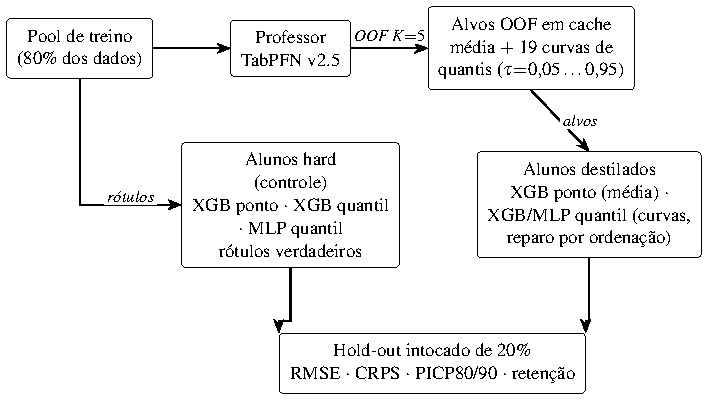
\includegraphics{images/tikz-cap7-1.pdf}
\caption{Pipeline de destilação distribucional: o professor rotula o
\emph{pool} fora de dobra e alunos de capacidade idêntica diferem
apenas no alvo de treino. Fonte: diagrama portado do artigo AI-2
(\texttt{latex/\allowbreak ai2/\allowbreak main.\allowbreak tex}).}
\label{fig:destil-pipeline}
\end{figure}

\subsection{Métricas}
\label{sec:destil-metricas}

Para a qualidade pontual, RMSE e MAE. Para a qualidade distribucional,
o \textbf{CRPS} (\emph{continuous ranked probability score}
\citep{gneiting2007}: a regra de pontuação própria que generaliza o
erro absoluto de predições pontuais para distribuições preditivas
completas; menor é melhor), estimado como duas vezes a média das
perdas \emph{pinball} sobre a grade de 19 quantis
\citep{gneiting2011} --- o estimador de grade padrão na prática de
previsão probabilística. Validamos esse estimador contra a forma
fechada gaussiana: ele carrega uma sobre-estimativa multiplicativa
quase constante de ${\sim}4$--5\% (razão 1,048 nos quatro cenários de
locação$\times$escala;
\texttt{results/\allowbreak distillation/\allowbreak crps\_\allowbreak grid\_\allowbreak gaussian\_\allowbreak validation.\allowbreak csv}),
aproximadamente independente de
locação e escala nos cenários testados, de modo que todas as
comparações internas e razões de retenção ficam preservadas --- mas os
valores absolutos de CRPS não devem ser comparados aos de outros
trabalhos. Para calibração, PICP80/90 (a fração dos alvos de teste
dentro do intervalo nominal de 80\%/90\%) com as larguras dos
intervalos. A métrica-síntese é a \textbf{retenção do gap de CRPS},
\begin{equation}
  \mathrm{ret} \;=\;
  \frac{\mathrm{CRPS}_{\mathrm{hard}} - \mathrm{CRPS}_{\mathrm{soft}}}
       {\mathrm{CRPS}_{\mathrm{hard}} - \mathrm{CRPS}_{\mathrm{professor}}},
\label{eq:destil-retencao}
\end{equation}
em que 1 significa que o aluno destilado recupera toda a vantagem do
professor sobre o seu próprio controle de rótulos verdadeiros, valores
negativos significam que a destilação prejudicou, e valores acima de 1
caracterizam o efeito \emph{born-again} --- o aluno supera o próprio
professor, o fenômeno que \citet{furlanello2018} documentam em redes;
o termo vem da compressão de \emph{ensembles} em árvores
\citep{breiman1996,vidal2020}, na qual o aluno apenas \emph{imita} o
comitê. A latência é medida em \us/linha no
\emph{hold-out} do benchmark (mediana de 5 passadas para os alunos; passada
única cronometrada para os professores, cujo custo por passada é de
minutos).

\subsection{Conjuntos de dados e infraestrutura}
\label{sec:destil-setup}

\begin{sloppypar}
O estudo usa os cinco conjuntos de regressão do benchmark
(\texttt{wine\_quality}, \texttt{california\_\allowbreak housing},
\texttt{online\_news}, \texttt{kin8nm}, \texttt{year\_\allowbreak prediction};
pools de 5,2 mil a 80 mil linhas) mais \textbf{quinze conjuntos} da
suíte OpenML-CTR23
\citep{fischer2023}, selecionados sob regra declarada ---
3 mil a 100 mil linhas, ids de versão fixados, e dois conjuntos da
suíte excluídos por vazamento de alvo descoberto na verificação (o
alvo é soma de atributos em \texttt{brazilian\_\allowbreak houses} e
\texttt{wave\_energy}). Uma versão anterior deste texto chamava os
quinze de ``pool elegível completo''; a auditoria externa de
23/11/2026 recontou a regra e encontrou \textbf{dezenove} elegíveis.
Os quatro ausentes, nomeados e com o status de cada um:
\texttt{white\_\allowbreak wine} (44971; subconjunto do
\texttt{wine\_\allowbreak quality} do núcleo),
o \texttt{california\_\allowbreak housing} \emph{contínuo} (44977;
versão não binarizada do conjunto do núcleo),
\texttt{superconductivity} (44964; à época da seleção
acreditava-se sobreposto ao núcleo, crença que a errata de 19/10
desfez --- e a omissão não foi revisitada) e
\texttt{naval\_\allowbreak propulsion\_\allowbreak plant} (44969; sem
justificativa registrada). A sensibilidade foi medida sob o mesmo
protocolo (um split, sementes $\{0,1,2\}$) e re-executada por nós: o
placar vai de 16/20 ($p=0{,}0059$) para \textbf{17/24}
($p=0{,}032$) com os quatro --- o destilado \emph{ganha} no
california contínuo ($+3{,}7\%$ de CRPS) e perde nos outros três ---
e para \textbf{16/22} ($p=0{,}026$) no recorte conservador que
exclui os dois de sobreposição real com o núcleo
(\texttt{white\_\allowbreak wine} e o próprio california contínuo,
que é uma \emph{vitória} do destilado); as duas derrotas grandes
(\texttt{white\_\allowbreak wine}, \texttt{superconductivity}) têm
29--36\% do teste com gêmeo exato no \emph{pool}, o mesmo mecanismo
de memorização de duplicatas do \texttt{wine\_\allowbreak quality},
enquanto a derrota no \texttt{naval} é genuína
(\texttt{results/\allowbreak distillation/\allowbreak
ctr23\_\allowbreak sensitivity.csv}; proveniência e limites em
\texttt{ctr23\_\allowbreak omitidos/\allowbreak PROVENANCE.md}). A
trajetória da fixação do pool ---
incluindo o corte interino não significativo com $N{=}15$ (teste de
sinal $p{=}0{,}059$) --- está na Seção~\ref{sec:destil-desenho}, com a
correção sequencial que ela exige.
Duas notas de identidade (errata de 19/10/2026, Seção~\ref{sec:met-datasets}):
o conjunto historicamente rotulado ``superconduct'' é o
\texttt{online\_news} (OnlineNewsPopularity; regressão contínua
legítima --- apenas o rótulo estava errado), e o
\texttt{california\_\allowbreak housing} é a variante com \textbf{alvo binarizado}
do \emph{tabular-benchmark} --- degenerada para afirmações
distribucionais; todos os resultados-manchete deste capítulo ganham,
por isso, análise de sensibilidade com esse conjunto excluído
(reportada junto a cada resultado). As partições são
idênticas às do benchmark --- \emph{hold-out} fixo de 20\% (semente 42) que
nenhuma etapa de seleção jamais observa --- com três sementes de aluno
em todo o estudo. O hardware é a mesma RTX~5080 (16~GB) dos capítulos
anteriores; os tetos de VRAM são tratados como medições, não como
incômodos, e reaparecem como achado na
Seção~\ref{sec:destil-fronteira}.
\end{sloppypar}

\section{A destilação pontual é refutada --- com qualquer professor}
\label{sec:destil-ponto}

O primeiro resultado é o negativo que o pré-registro se comprometeu a
reportar. Nos 20 conjuntos, o aluno pontual treinado nas médias do
professor supera o seu controle de rótulos verdadeiros em apenas
\textbf{4}; H1 é refutada já nos cinco conjuntos centrais. A objeção
natural --- ``o professor não era forte o suficiente'' --- foi testada
diretamente, replicando o experimento com o TabFM, cujo gap de âncora
(a vantagem de RMSE do professor sobre o controle compartilhado, o
denominador da retenção) é quase $6\times$ o do TabPFN no
\texttt{california\_\allowbreak housing} (conjunto da errata): 0,028 contra
0,005 de RMSE. O quadro não
muda: somente as duas células \emph{soft} do \texttt{california}
superam o controle, com melhor retenção intra-pipeline de 0,11
(california/misto), e as oito células restantes ficam no nível do
controle ou abaixo. Em \emph{pool} completo, um GBDT ajustado extrai dos
rótulos brutos tanta acurácia pontual quanto das opiniões do professor
sobre eles.

Surpreendentemente, um resquício de ganho aparecia nos experimentos
exploratórios menores --- e o contraste entre execuções \emph{smoke} e
piloto sugeriu a hipótese de que o ganho pontual é um fenômeno de
poucos dados. Investigamos com uma varredura de tamanho de \emph{pool} (caps
de 800, 2.000 e 8.000 linhas): há um ganho genuíno de poucos dados no
\texttt{wine\_quality} ($\Delta = +0{,}026$ em $n{=}800$), que
desaparece a partir de $n{=}2.000$ e \emph{não} replica no
\texttt{california\_\allowbreak housing}. Atribuímos o resquício, portanto, a um
moderador de poucos dados dependente do conjunto, e o reportamos como
observação, não como efeito geral.

Essa varredura é também a chave da reconciliação com a colisão
parcial da Seção~\ref{sec:destil-novidade}: \citet{jeong2026} reportam
ganhos de destilação pontual em regressão com professores mais novos
(TabPFN~v3 e TabICLv2), transferência por erro quadrático e avaliação
apenas de RMSE, sob protocolo e suítes distintos --- e com uma receita
que difere da nossa em eixos que não replicamos (rotulagem com
contexto completo, expansão por consultas sintéticas, aluno treinado
só em predições do professor). Nossa varredura
oferece uma hipótese de moderação para o contraste --- ganho residual
restrito a \emph{pools} pequenos ---, e o nosso
negativo é escopado com precisão: tamanhos de \emph{pool} realistas (3 mil a
100 mil linhas), capacidade do aluno fixada pelo tuning do benchmark.
As duas leituras são compatíveis; a reconciliação exata é proposta,
não demonstrada.

\emph{A destilação pontual falha em escala de \emph{pool} realista,
independentemente do professor.} O aluno pontual destilado supera o
controle de rótulos verdadeiros em apenas 4 de 20 conjuntos; a
replicação com um professor quase $6\times$ mais forte (gap de âncora
0,028 vs.\ 0,005 de RMSE no \texttt{california\_\allowbreak housing}) não altera o
quadro, e a varredura de \emph{pool} mostra que o ganho residual é um
fenômeno de poucos dados ($n \leq 800$) em alguns conjuntos apenas.
H1 é refutada; o que o professor sabe sobre a \emph{média} o aluno
aprende sozinho dos dados.

\section{A destilação distribucional funciona --- onde o professor tem
vantagem}
\label{sec:destil-dist}

Transferir as curvas de quantis do professor --- e não sua média ---
muda o desfecho. A Tabela~\ref{tab:destil-retencao} apresenta o
resultado central do capítulo sobre o \emph{pool} completo de 20 conjuntos:
para cada um, a retenção do gap de CRPS
(Eq.~\ref{eq:destil-retencao}), a vantagem absoluta do professor sobre o
controle e a melhoria absoluta do aluno destilado, todas em unidades
do alvo. Na tabela, $n$ é o tamanho do \emph{pool} de treino após o
\emph{hold-out} de 20\%, e \texttt{diamonds\_real} é o verdadeiro
conjunto diamonds do OpenML, incluído quando a errata de rotulagem
descrita no Capítulo~\ref{chap:metodologia} foi retificada.

\begin{table}[htb]
\centering
\caption{Retenção do gap de CRPS do aluno multiquantil destilado nos
20 conjuntos (média de 3 sementes). Fonte:
\texttt{results/\allowbreak distillation/\allowbreak paper\_\allowbreak retention.\allowbreak csv}.}
\label{tab:destil-retencao}
\small
\begin{tabular}{llrrrr}
\toprule
Conjunto & Origem & $n$ & Retenção & Vant.\ professor & $\Delta$CRPS \\
\midrule
pumadyn32nh            & CTR23  & 6.553  & $+1{,}057$ & 0,001  & $+0{,}0006$ \\
california\_housing    & núcleo & 16.507 & $+0{,}644$ & 0,111  & $+0{,}072$ \\
abalone                & CTR23  & 3.341  & $+0{,}595$ & 0,095  & $+0{,}056$ \\
fps\_benchmark         & CTR23  & 19.699 & $+0{,}523$ & 0,152  & $+0{,}080$ \\
cpu\_activity          & CTR23  & 6.553  & $+0{,}500$ & 0,233  & $+0{,}117$ \\
cps88wages             & CTR23  & 22.524 & $+0{,}465$ & 0,345  & $+0{,}160$ \\
year\_prediction       & núcleo & 80.000 & $+0{,}419$ & 0,311  & $+0{,}130$ \\
online\_news           & núcleo & 31.715 & $+0{,}255$ & 0,006  & $+0{,}0015$ \\
sarcos                 & CTR23  & 39.146 & $+0{,}225$ & 0,474  & $+0{,}107$ \\
kings\_county          & CTR23  & 17.290 & $+0{,}213$ & 7.253,4 & $+1.547$ \\
grid\_stability        & CTR23  & 8.000  & $+0{,}170$ & 0,003  & $+0{,}0004$ \\
kin8nm                 & núcleo & 6.553  & $+0{,}128$ & 0,030  & $+0{,}0039$ \\
physiochemical\_protein& CTR23  & 36.584 & $+0{,}086$ & 0,573  & $+0{,}049$ \\
video\_transcoding     & CTR23  & 55.027 & $+0{,}086$ & 0,092  & $+0{,}0079$ \\
space\_ga              & CTR23  & 2.485  & $+0{,}078$ & 0,011  & $+0{,}0009$ \\
miami\_housing         & CTR23  & 11.145 & $+0{,}016$ & 4.117,4 & $+67{,}7$ \\
health\_insurance      & CTR23  & 17.817 & $-0{,}255$ & 0,150  & $-0{,}038$ \\
diamonds\_real         & CTR23  & 43.152 & $-0{,}315$ & 9,422  & $-2{,}97$ \\
wine\_quality          & núcleo & 5.197  & $-0{,}970$ & 0,039  & $-0{,}037$ \\
fifa                   & CTR23  & 15.342 & $-1{,}287$ & 42,95  & $-55{,}3$ \\
\bottomrule
\end{tabular}
\end{table}

A leitura agregada: a retenção é positiva em \textbf{16 de 20}
conjuntos, com mediana $+0{,}19$, máximo $+1{,}06$
(\texttt{pumadyn32nh} --- um aluno \emph{born-again} que supera o
próprio professor) e sequência de sucessos grandes em
\texttt{california\_\allowbreak housing} ($+0{,}64$), \texttt{abalone}
($+0{,}59$), \texttt{fps\_benchmark} ($+0{,}52$) e
\texttt{cpu\_activity} ($+0{,}50$). Os dois instrumentos frequentistas
rejeitam a hipótese nula ao nível de 5\%, ambos unilaterais conforme a
hipótese direcional (teste de sinal
$p = 0{,}006$ na leitura ingênua e $p \approx 0{,}019$ sob a correção
sequencial do desenho em duas etapas --- o instrumento foi fixado após
a leitura intermediária, Seção~\ref{sec:destil-desenho};
Wilcoxon $p = 0{,}045$ --- limítrofe, e na versão
bilateral ($p = 0{,}090$) não rejeitaria: por isso a manchete repousa
no teste de sinal e na mediana) e o teste bayesiano de postos
sinalizados \citep{benavoli2017} coloca 0,96 da probabilidade
posterior na região de retenção positiva (fração de amostras
posteriores em que a região é a mais provável, a convenção de
Benavoli et al.; a massa posterior esperada, $E[\theta]$, é 0,70) com
região de equivalência prática (ROPE) de
$\pm 0{,}05$ --- estável em 0,95--0,96 (e $E[\theta]$ em 0,63--0,71)
na varredura de ROPE de 0,02 a
0,10. A sensibilidade à errata do \texttt{california\_\allowbreak housing} (alvo
binarizado; Seção~\ref{sec:met-datasets}) é reportada com a mesma
proeminência: excluído o conjunto degenerado, a retenção fica positiva
em 15 de 19, com mediana $+0{,}17$, teste de sinal $p = 0{,}010$ e
IC de \emph{bootstrap} ainda inteiramente positivo $[0{,}08; 0{,}42]$
--- mas o Wilcoxon unilateral passa a $p = 0{,}067$ e deixa de
rejeitar a 5\%
(\texttt{results/\allowbreak distillation/\allowbreak sensitivity\_\allowbreak california.\allowbreak csv}). A
conclusão qualitativa não depende do conjunto; o par de instrumentos
fica com o sinal significativo e o Wilcoxon marginal.

A honestidade da leitura exige quatro ressalvas, e elas estão embutidas
na própria tabela. Primeiro, a retenção é uma \emph{razão}, e fica
instável quando a vantagem absoluta do professor é pequena: o caso
\emph{born-again} do \texttt{pumadyn32nh} cavalga uma vantagem de
apenas $0{,}0006$ de CRPS (e \texttt{online\_news} e
\texttt{grid\_\allowbreak stability} são análogos) --- por isso a tabela reporta a
melhoria absoluta ao lado da razão, e por isso a manchete do capítulo
se apoia no \textbf{teste de sinal e na mediana}, que são livres de
escala. O rótulo de ``sucesso grande'', por sua vez, exige leitura
relativa: o \texttt{cps88wages}, cuja melhoria absoluta de $+0{,}160$
parece expressiva, opera sobre CRPS de ${\sim}160$ --- o ganho
relativo é de $0{,}1\%$ e o \emph{bootstrap} pareado por linhas do
teste não o distingue de zero;
entre os sucessos absolutos ficam \texttt{year\_\allowbreak prediction}
($+0{,}130$; vitória clara no \emph{bootstrap}, $+2{,}9\%$ com IC95
$[2{,}6;\,3{,}2]$) e \texttt{cpu\_activity} ($+0{,}117$). O
\emph{bootstrap} por linhas, aliás, é a análise de incerteza por
conjunto que o pré-registro de 15/07 prometia e que faltava: refeita
em 23/11 (B=10.000, alunos re-treinados nas três sementes, CRPS por
linha do \emph{hold-out}), ela dá à manchete a sua leitura mais
honesta --- \textbf{13 vitórias claras} (IC95 inteiramente positivo),
\textbf{4 empates} (\texttt{cps88wages}, \texttt{miami\_\allowbreak housing},
\texttt{space\_ga}, \texttt{health\_\allowbreak insurance}) e
\textbf{3 derrotas claras}: o teste de sinal conta empates ruidosos
como vitórias, e o 16/20 deve ser lido como ``13 claras $+$ 3
limítrofes''
(\texttt{results/\allowbreak distillation/\allowbreak bootstrap\_\allowbreak lines.csv}).
Segundo, o segundo maior sucesso
da tabela, o \texttt{california\_\allowbreak housing} ($+0{,}64$; $+0{,}072$ de
CRPS), é exatamente o conjunto de alvo binarizado da errata: ali o
``ganho distribucional'' é calibração de uma Bernoulli, não regressão
contínua --- a análise de sensibilidade acima o exclui por isso;
onde o conjunto reaparece em exemplos (a fronteira de \emph{serving},
os custos por linha), o rótulo da errata o acompanha, e nenhuma
manchete repousa sobre ele. Terceiro, nenhuma retenção é exatamente zero, mas
positivos quase nulos como o \texttt{miami\_housing} ($+0{,}016$)
contam como sucesso sob o teste de sinal --- a varredura de ROPE acima
delimita o efeito de tratá-los como equivalências. Quarto, as
falhas são diagnosticáveis --- mas cada uma pela própria causa, e a
auditoria externa de 23/11/2026 derrubou o diagnóstico ``comum'' que
uma versão anterior deste texto oferecia. No \texttt{wine\_quality},
a causa é um artefato do conjunto: 27,6\% do teste tem gêmeo exato de
covariáveis no \emph{pool} (o conjunto original traz 1.179 linhas
duplicadas), o controle \emph{pinball} memoriza os gêmeos e o aluno,
treinado nas curvas suavizadas do professor, não --- nas linhas
\emph{sem} gêmeo o destilado vence por $+3{,}0\%$ de CRPS, e no
conjunto deduplicado ($n=5.318$, professor re-rotulado OOF) o
destilado vence nas três sementes, com ganho de $+0{,}85\%$ e
retenção $+0{,}10$
(\texttt{results/\allowbreak distillation/\allowbreak wine\_\allowbreak dedup.csv});
a ``derrota'' publicada é memorização de duplicatas, não limitação da
destilação, e permanece na tabela porque o conjunto original é o da
população registrada. O \texttt{health\_\allowbreak insurance}, descrito em
versão anterior como alvo de escala de preço, tem na verdade por alvo
\texttt{whrswk} --- horas trabalhadas por semana, com 29,9\% de zeros
e assimetria \emph{negativa} ($-0{,}34$) --- e sua retenção vai de
$-0{,}26$ (herdado) a $+0{,}65$ (re-tunado): uma falha sensível à
configuração, não um efeito de escala
(\texttt{results/\allowbreak distillation/\allowbreak retune\_\allowbreak analysis.csv}).
Restam \texttt{fifa} e \texttt{diamonds\_\allowbreak real} como as falhas
genuínas em alvos de escala de preço --- e, para elas, a
Seção~\ref{sec:destil-regra} mostra que a hipótese da cauda pesada
não se confirma.

A qualidade transferida não é só o CRPS agregado: a calibração
acompanha --- e, num caso, excede --- a transferência, como as curvas
de confiabilidade da Seção~\ref{sec:destil-oof}
(Figura~\ref{fig:destil-calibration}) mostram em detalhe. A segunda
cláusula de H2, porém, recebe aqui o veredito explícito que a paridade
com as refutações exige: a exigência pré-registrada de cobertura a
$\pm 5$~p.p.\ do nominal \textbf{não é cumprida} pelo aluno destilado
puro --- o PICP80 fica dentro da faixa em 10 dos 20 conjuntos (e em 2
dos 5 centrais) --- de modo que H2 é confirmada apenas na cláusula de
CRPS; o remédio é medido no piloto conformal
(Seção~\ref{sec:destil-oof}), que conserta a cobertura --- no critério
de a distância ao nominal diminuir --- em 5/5 conjuntos no braço
\emph{soft} e 3/5 no \emph{hard}, sem mover o CRPS.

\emph{A destilação distribucional retém mediana de 19\% da
vantagem de CRPS do professor, positiva em 16 de 20 conjuntos.} A
transferência das 19 curvas de quantis para um aluno multiquantil é
positiva em 16/20 conjuntos (teste de sinal unilateral $p=0{,}006$,
$p \approx 0{,}019$ sob a correção sequencial da
Seção~\ref{sec:destil-desenho};
Wilcoxon unilateral
$p=0{,}045$ na população de 20 --- na sensibilidade de 19 conjuntos,
sem o alvo binarizado da errata, o Wilcoxon vai a $p=0{,}067$, acima
do corte de 5\%, enquanto o teste de sinal mantém 15/19,
$p=0{,}010$; probabilidade posterior bayesiana 0,96 em ROPE
$\pm 0{,}05$, com $E[\theta]=0{,}70$), com
máximo de $+1{,}06$ --- um aluno \emph{born-again}, com a ressalva de
que esse caso repousa sobre vantagem absoluta de $0{,}0006$ de
CRPS --- a latências de microssegundos. As quatro falhas são
discutidas uma a uma na
Seção~\ref{sec:destil-regra}, com os diagnósticos que a análise por
linhas e o teste de deduplicação sustentam --- e sem o diagnóstico
comum que uma versão anterior deste texto alegava.

\section{A fronteira de \emph{serving}: destilar, comprimir ou reduzir
ensemble}
\label{sec:destil-fronteira}

A retenção diz o que o aluno preserva; não diz quando ele é a escolha
certa contra as alternativas de engenharia que um praticante tem à
mão. Para responder H3, medimos acurácia e latência de \emph{todas} as
estratégias nos mesmos hold-outs, em três conjuntos de vantagem
positiva (um deles, o \texttt{california\_\allowbreak housing}, é o conjunto de
alvo binarizado da errata --- os números valem como medição de
latência$\times$CRPS, mas o \texttt{year\_\allowbreak prediction} é a vitrine
distribucional legítima da fronteira): o TabPFN com contexto subamostrado para
\{1 mil, 5 mil, 10 mil, 25 mil, completo\} (o braço ``comprimir
contexto'', na variante simples de subamostragem --- CRUMB
\citep{crumb2026} é o método representativo desse braço na
literatura); o TabPFN com 1/4/8 membros de \emph{ensemble} (o braço ``reduzir
\emph{ensemble}''); os alunos destilados e de controle (o braço
``destilar''); e o TabFM de contexto completo como âncora de acurácia
(4.905--394.301~\us/linha). A Figura~\ref{fig:destil-pareto} apresenta
a fronteira resultante: o eixo de latência é \emph{logarítmico} ---
distâncias horizontais iguais são fatores multiplicativos iguais ---,
melhor é abaixo e à esquerda, e o que importa é a distância vertical
entre o aluno destilado e a curva do professor na latência medida mais
próxima.

\begin{figure}[htb]
\centering
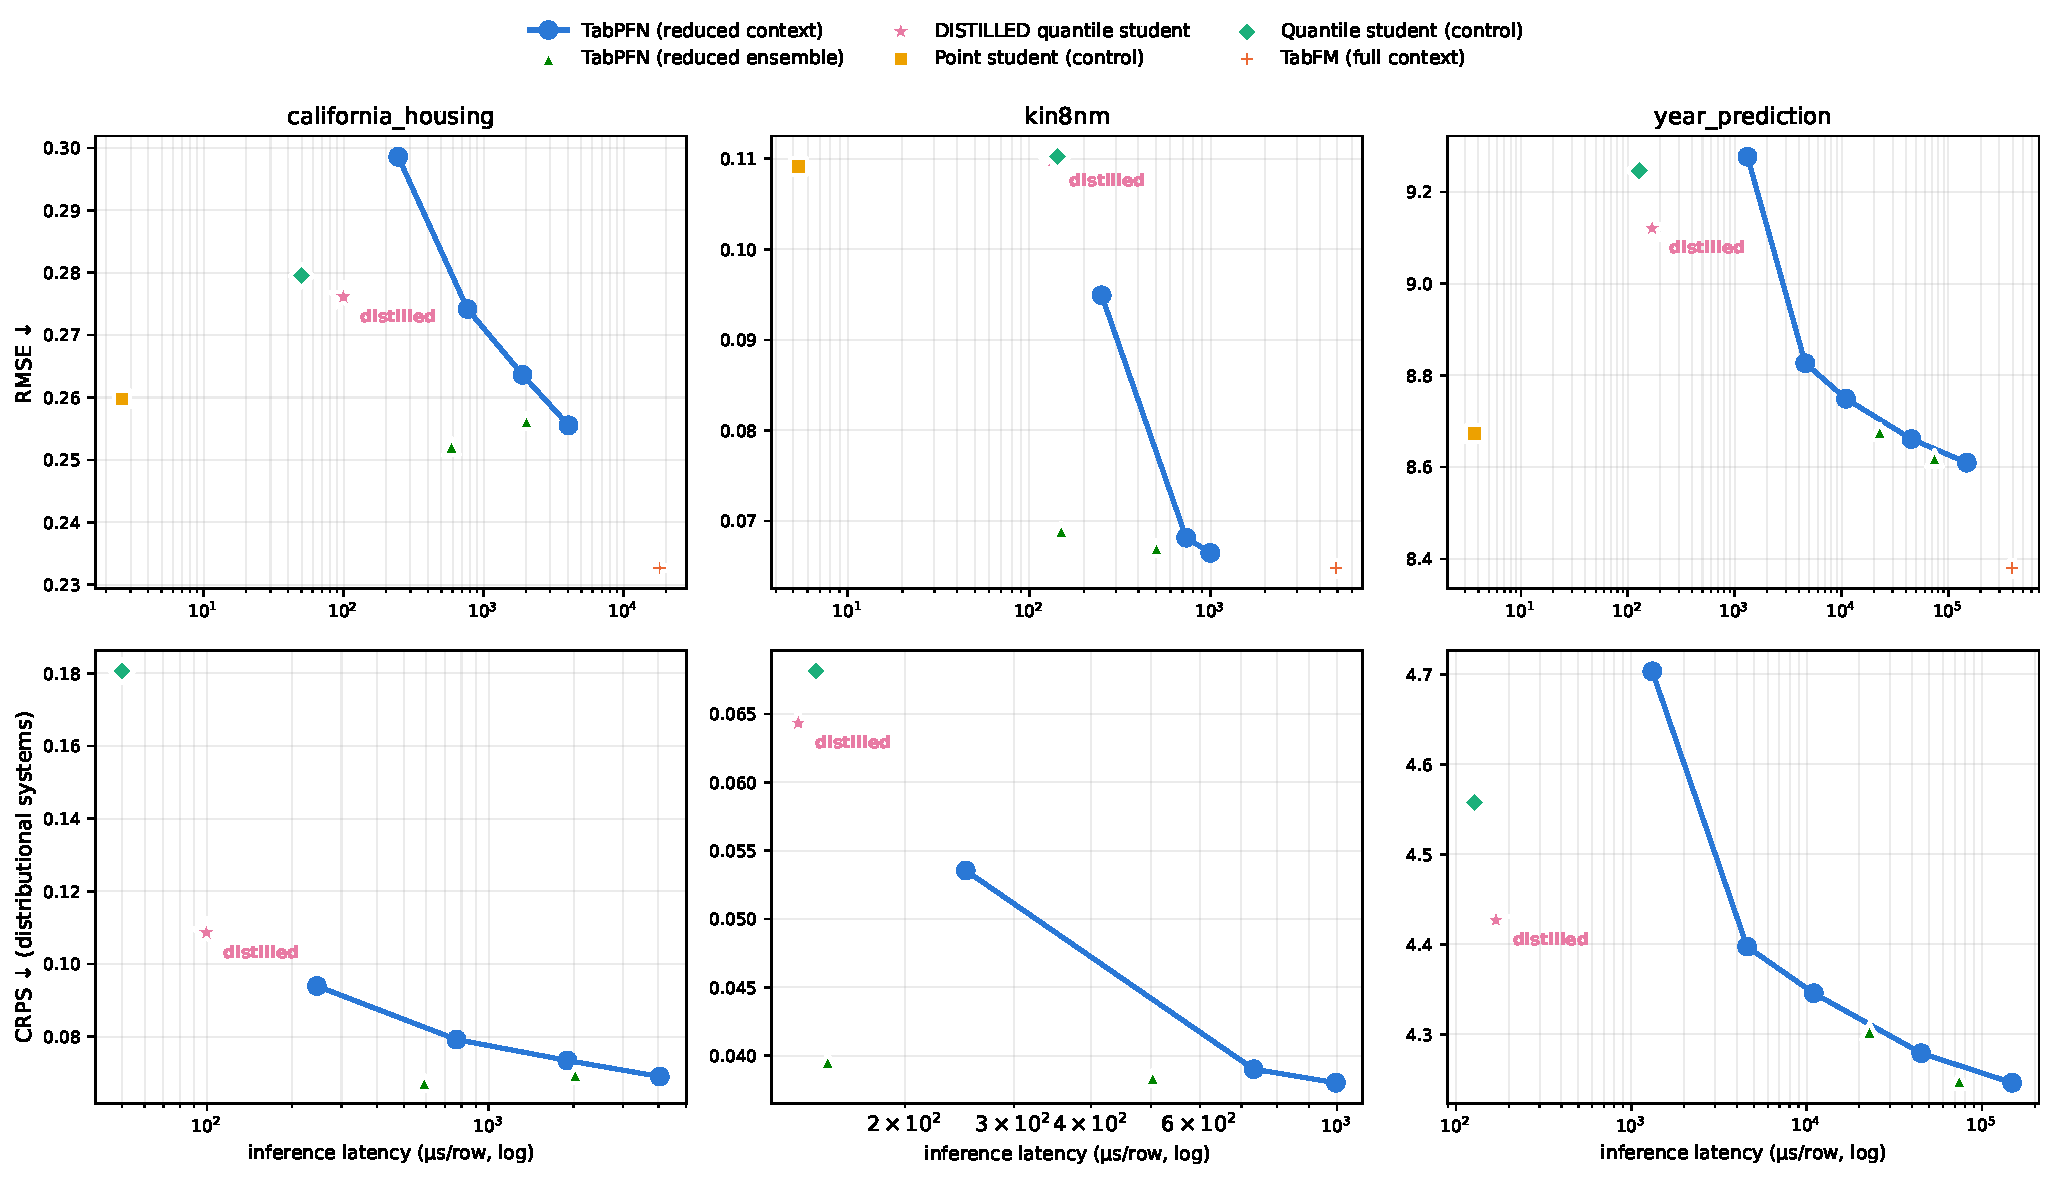
\includegraphics[width=\linewidth]{images/pareto_distill_en.pdf}
\caption{Fronteira destilar $\times$ comprimir $\times$ reduzir
\emph{ensemble}: RMSE (acima) e CRPS (abaixo) contra latência de
inferência em três conjuntos de vantagem positiva (rótulos internos em
inglês, conforme a figura do artigo AI-2). Fonte:
\texttt{results/\allowbreak distillation/\allowbreak pareto.\allowbreak csv}.}
\label{fig:destil-pareto}
\end{figure}

A figura separa três regimes. No plano \textbf{pontual} (linha
superior), o aluno de controle com rótulos verdadeiros já ocupa o
regime rápido (2,6--5,3~\us/linha) --- é a refutação de H1 tornada
visível: não há nada que a destilação pontual pudesse acrescentar ali.
No plano \textbf{distribucional} (linha inferior), abaixo de
${\sim}250$~\us/linha no \texttt{california\_\allowbreak housing} e de
${\sim}1.300$~\us/linha no \texttt{year\_\allowbreak prediction}, as estratégias
derivadas do professor deixam os alunos sozinhos, e o destilado é o
CRPS-ótimo entre eles (o E1 mediria depois que a QRF nativa também
habita esse regime --- e no \texttt{california\_\allowbreak housing} o supera;
Seção~\ref{sec:destil-e1}): CRPS 0,109 a
99~\us/linha onde a configuração mais barata do professor precisa de
245~\us/linha para 0,094 --- $2{,}5\times$ a latência do aluno --- no
\texttt{california\_\allowbreak housing}; e CRPS 4,43 a 169~\us/linha onde a
configuração mais barata do professor que o supera custa
4.576~\us/linha --- $27\times$ a latência --- no
\texttt{year\_\allowbreak prediction}.

O terceiro conjunto inverte o quadro --- e a inversão é instrutiva. No
\texttt{kin8nm}, a vantagem do professor é pequena ($+0{,}030$ de CRPS)
e um TabPFN de \emph{um único membro} entrega CRPS 0,040 a
150~\us/linha --- essencialmente a latência do aluno. Ali, a alavanca
certa é a redução de \emph{ensemble}, não a destilação: é a contraparte, no
nível da fronteira, da regra de decisão da
Seção~\ref{sec:destil-regra} --- quando a vantagem do professor é
pequena, o menu de engenharia barata resolve antes que a destilação
entre em cena.

O veredito de H3, que uma versão anterior deixava implícito, fica
explícito: \textbf{confirmada com escopo estreito}. No
\texttt{year\_\allowbreak prediction} o aluno destilado é
Pareto-dominante no sentido forte --- CRPS melhor que o do professor
mais subamostrado (4,43 contra 4,70) a $7{,}8\times$ menos latência;
no \texttt{california\_\allowbreak housing} a faixa existe, mas é a
banda abaixo de 245~\us\ em que nenhuma configuração do professor
opera (e que a QRF nativa ocupa com CRPS melhor, como o E1 mediria);
no \texttt{kin8nm} a hipótese \emph{falha} --- a redução de
\emph{ensemble} entrega a latência do aluno com CRPS muito melhor.
H3 vale, portanto, onde a vantagem do professor é grande, e é
substituída pela engenharia barata onde é pequena --- a mesma
condição da regra de decisão.

Dois achados colaterais têm valor independente. Primeiro, reduzir o
\emph{ensemble} do TabPFN de 8 para 1 membro \emph{melhorou} o RMSE no
\texttt{california\_\allowbreak housing} (conjunto da errata; 0,2521 contra
0,2555) a um sétimo da
latência --- a redução de \emph{ensemble} é uma primeira alavanca subestimada,
às vezes gratuita. Segundo, a última duplicação de contexto
(25 mil $\to$ 50 mil) no \texttt{year\_\allowbreak prediction} exige o modo de
economia de memória da biblioteca na GPU de 16~GB e custa
$3{,}3\times$ a latência (148,6 contra 45,1~ms/linha) por um ganho de
RMSE de 0,05: em GPUs de porte comum, o professor de contexto completo
não se paga.

\emph{Onde a vantagem do professor é grande, o aluno destilado é,
entre as estratégias derivadas do professor, o sistema distribucional
CRPS-ótimo abaixo da configuração competitiva
mais barata dele; onde é pequena, reduzir o \emph{ensemble} basta ---
e, antes de qualquer uma, teste-se o nativo clássico do E1.} Na
fronteira medida de ponta a ponta, a configuração mais barata do
professor que supera o aluno destilado custa $2{,}5\times$ a latência
dele no \texttt{california\_\allowbreak housing} e $27\times$ no
\texttt{year\_\allowbreak prediction}; no \texttt{kin8nm}, de vantagem pequena, um
professor de um membro já opera à latência do aluno. Colaterais: 1
membro do TabPFN $\approx$ 8 membros a 1/7 da latência, e a última
duplicação de contexto é desproporcionalmente cara em GPUs de 16~GB.

\section{Por que rotular out-of-fold: calibração, não acurácia}
\label{sec:destil-oof}

A literatura de classificação \citep{pocketfm2026} estabelece que
rótulos do professor \emph{in-sample} colapsam em direção ao one-hot e
devem ser evitados. A regressão, mostramos, se comporta de outro modo
--- e a diferença só aparece quando o confundidor é removido. Nossa
ablação de três regimes compara: OOF (contexto de 80\%, sem
vazamento), \emph{in-sample} com o \emph{mesmo} contexto de 80\% (com
vazamento, contexto idêntico) e \emph{in-sample} com contexto
completo. O desenho desconfunde vazamento de tamanho de contexto ---
exatamente o que a comparação usual OOF vs.\ \emph{in-sample} não
separa.

O resultado: o vazamento, isolado, \emph{não} degrada acurácia --- o
RMSE até melhora nos quatro conjuntos testados, e o CRPS em três ---
e o tamanho do contexto contribui pouco (embora, no
\texttt{wine\_quality}, custe 5,9~p.p.\ adicionais de cobertura). O
dano concentra-se na \textbf{cobertura de intervalos}: a contexto
idêntico, alunos rotulados \emph{in-sample} perdem de 0,5 a 5,1~p.p.\
de PICP80 em todos os quatro conjuntos --- artefato
\texttt{ablation\_\allowbreak insample.\allowbreak csv} em \texttt{results/\allowbreak distillation/}. A
mecânica é
legível: o professor é superconfiante nas linhas que tem em contexto, e
essa superconfiança --- invisível às métricas de acurácia ---
transfere-se ao aluno como intervalos estreitos demais. Em regressão,
a rotulagem OOF é uma salvaguarda de \emph{calibração}, não de
acurácia --- um refinamento desconfundido do achado de classificação.

A Figura~\ref{fig:destil-calibration} fecha o eixo da calibração com
as curvas de confiabilidade dos sistemas distribucionais ---
prometidas na Seção~\ref{sec:destil-dist}: para cada nível nominal
$\tau$, a fração empírica de alvos abaixo do quantil $\tau$ predito,
com a diagonal como calibração perfeita. A regra de leitura correta
--- a mesma da Figura~\ref{fig:quantis-cobertura} --- é por nível:
curva acima da diagonal num $\tau$ significa quantil predito
\emph{alto} demais naquele nível; a cobertura de um intervalo central
$[q_{0{,}10}, q_{0{,}90}]$ é a \emph{diferença} entre as frações nos
dois níveis, de modo que uma curva mais íngreme que a diagonal no
centro indica intervalos estreitos demais (subcobertura) --- não
existe um atalho ``acima = sobre-cobre'' válido para a curva inteira,
como uma versão anterior desta legenda sugeria. No \texttt{california\_\allowbreak housing},
o controle de rótulos verdadeiros satura em sobrecobertura extrema e o
professor exibe a forma em S de caudas mal calibradas, enquanto o
aluno destilado é o mais próximo da diagonal; no \texttt{cpu\_activity},
os três sistemas são bem calibrados e o destilado permanece
competitivo. A transferência de curvas com reparo por ordenação atua
como regularizador de calibração, não como cópia --- e uma ablação
dedicada isola o componente: o reparo melhora ou empata o CRPS em 20
de 20 conjuntos nos dois braços --- melhora estrita em 20 de 20 no
braço \emph{hard} e 18 de 20 no \emph{soft} (dois empates exatos) ---, mas com
efeito mediano inferior a 1\%, de modo que nenhuma conclusão do
capítulo depende dele (Apêndice~\ref{sec:app-abl-sort}).

\begin{figure}[htb]
\centering
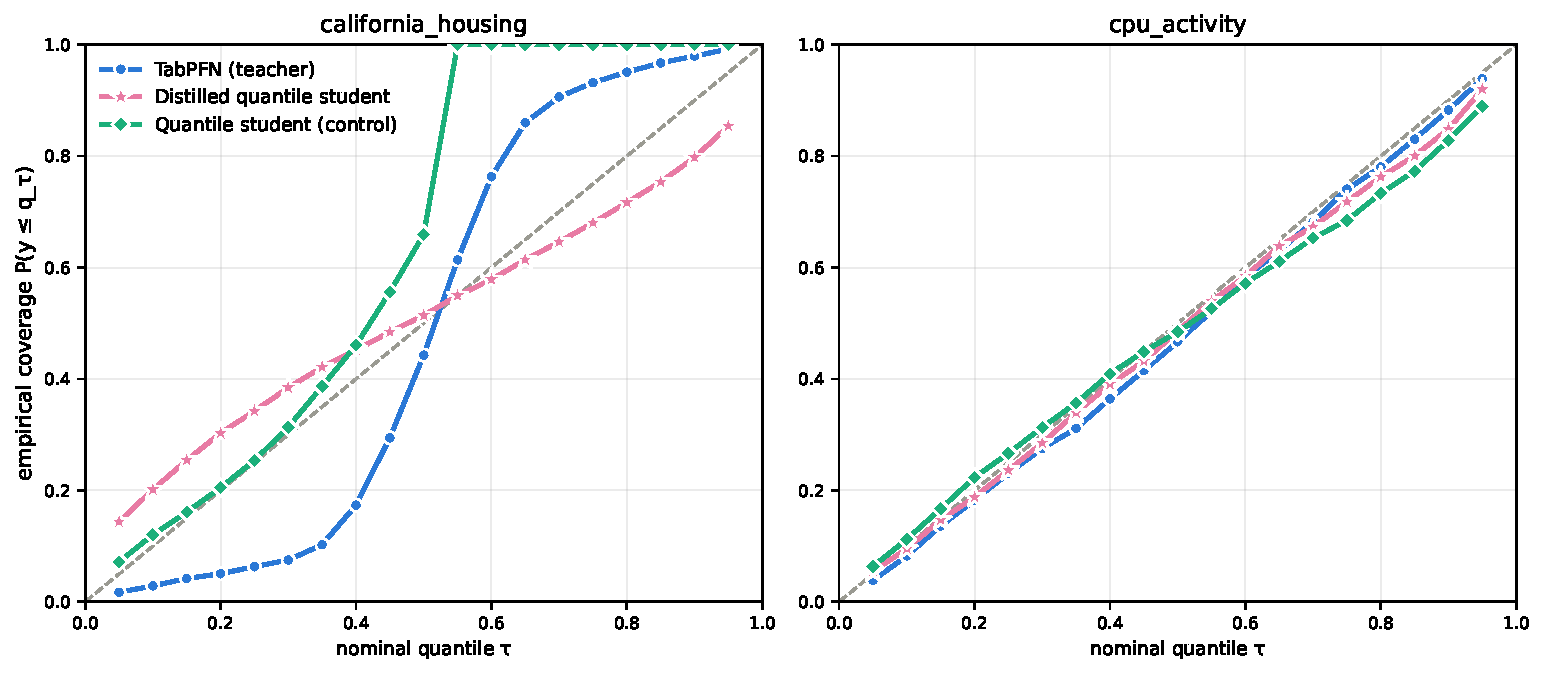
\includegraphics[width=\linewidth]{images/calibration_distill_en.pdf}
\caption{Confiabilidade no \emph{hold-out} (\texttt{california\_housing},
\texttt{cpu\_activity}): professor TabPFN, aluno destilado e controle,
em rótulos ingleses do artigo AI-2; a mecânica dos eixos é a da
Figura~\ref{fig:quantis-cobertura}. Fonte: \texttt{scripts/\allowbreak plot\_\allowbreak calibration.\allowbreak py}.}
\label{fig:destil-calibration}
\end{figure}

\emph{A rotulagem out-of-fold protege a calibração do aluno,
não sua acurácia.} Com contexto idêntico, rótulos \emph{in-sample} não
degradam RMSE nem CRPS, mas erodem a cobertura de intervalos em 0,5 a
5,1~p.p.\ de PICP80 nos quatro conjuntos testados: a superconfiança
em contexto do professor transfere-se ao aluno. E a destilação chega a
\emph{melhorar} a calibração num dos dois critérios: no
\texttt{california\_\allowbreak housing}, o aluno
destilado tem o menor desvio médio da diagonal entre os três sistemas
--- mas, no critério de cobertura do intervalo central, ele
\emph{subcobre} (PICP80 de 0,596, contra sobrecobertura de
${\sim}0{,}94$ do professor): ``mais bem calibrado'' vale no primeiro
critério, não no segundo, e é o passo conformal que fecha a cobertura
(com as ressalvas da errata: ali o alvo é binarizado, e ``calibração''
é a de uma Bernoulli).

Resta a objeção simétrica: se o ganho fosse \emph{apenas} calibração,
uma correção conformal barata sobre o controle de rótulos verdadeiros
o alcançaria. Um piloto declarado (5 conjuntos, 3 sementes,
\emph{split-conformal} por quantil nos dois braços) responde que não:
a conformalização conserta a cobertura --- no critério de a distância
ao nominal diminuir --- em 5/5 conjuntos no braço \emph{soft} e 3/5 no
\emph{hard} (as exceções: o california-\emph{hard}, que já sobre-cobria
e cuja cobertura a conformalização afasta do nominal, com distância de
PICP80 de $8{,}06$ para $9{,}63$~p.p., e o cps88wages-\emph{hard},
que já estava a menos de 1~p.p.\ do nominal e se move menos de
1~p.p.), mas
move o CRPS em menos de 1\% --- a vantagem de forma do destilado
sobrevive intacta à correção. Conformalização compra calibração;
destilação compra forma (Apêndice~\ref{sec:app-pilot-conformal}).

\section{E1 --- baselines distribucionais clássicos: o nativo forte
posto à prova}
\label{sec:destil-e1}

O artigo AI-2 declara, entre suas limitações, que baselines
distribucionais clássicos fora das famílias comparadas --- NGBoost
\citep{duan2020} e florestas aleatórias quantílicas (QRF)
\citep{meinshausen2006} --- não
foram incluídos: os alunos-quantil de rótulos verdadeiros fazem o
papel de \emph{baseline} distribucional nativo \emph{dentro} das famílias
testadas. A limitação esconde um possível confundidor: se um aluno
nativo clássico forte fechasse sozinho o gap que atribuímos à
destilação, a contribuição inteira estaria superdimensionada. Esta
seção fecha essa lacuna com o experimento E1, pré-registrado em
\texttt{docs/\allowbreak desenho-\allowbreak melhorias-\allowbreak finais.\allowbreak md} em 05/10/2026, \emph{antes}
da execução, conforme o contrato de conduta do programa.

\subsection{Desenho pré-registrado}
\label{sec:destil-e1-desenho}

Duas hipóteses falsificáveis foram fixadas, com critérios de
interpretação registrados para \emph{ambos} os desfechos:

\begin{itemize}
  \item \textbf{H-B1:} na maioria dos 20 conjuntos, o CRPS do aluno
    destilado é menor ou igual ao do melhor \emph{baseline} clássico (teste
    de sinal unilateral; $\alpha = 0{,}05$);
  \item \textbf{H-B2:} os baselines clássicos não alteram a leitura da
    fronteira --- suas latências são de microssegundos (o \emph{tier} dos
    alunos), logo competem com o aluno destilado em acurácia, não em
    custo.
\end{itemize}

Os critérios pré-fixados (\emph{gates}): se H-B1 confirmasse, a regra de decisão ganharia a nota ``um
nativo clássico forte não substitui a destilação onde a vantagem do
professor é grande''; se refutasse, \emph{todas} as alegações de vantagem
do aluno destilado seriam reescopadas nos artigos e nesta dissertação,
com o resultado negativo reportado com a mesma proeminência. O
protocolo é idêntico ao do restante do capítulo --- mesmos 20
conjuntos, mesmas partições (\emph{hold-out} de 20\%, semente 42), 3 sementes, o
mesmo estimador de CRPS sobre a grade de 19 quantis --- com uma
assimetria declarada no próprio pré-registro: o NGBoost (distribuição
Normal, parada antecipada em validação de 10\% do \emph{pool}) e a QRF
(quantis nativos nas mesmas 19~$\tau$) rodam com hiperparâmetros
\emph{default} documentados, \emph{sem} tuning específico, de modo que a
interpretação se limita a ``\emph{default} forte''. Um adendo datado do mesmo
dia registra a única decisão de execução: o pacote da QRF não aceita
valores faltantes (presentes em 3 conjuntos da CTR23; o NGBoost os
trata nativamente), e adotou-se imputação por mediana ajustada no \emph{pool}
e aplicada ao teste, somente no caminho da QRF --- política simples,
sem vazamento, declarada.

\subsection[Resultados: 17 de 20, com três reveses
instrutivos]{Resultados: 17 de 20 para o aluno destilado --- com três
reveses instrutivos}
\label{sec:destil-e1-resultados}

\begin{sloppypar}
Todos os números a seguir foram recomputados do artefato de análise
\texttt{baselines\_\allowbreak analysis.\allowbreak csv} (em
\texttt{results/\allowbreak distillation/}), que o script
\texttt{analyze\_\allowbreak baselines.\allowbreak py} agrega do artefato bruto
\texttt{classical\_\allowbreak baselines.\allowbreak csv}. \textbf{H-B1 é confirmada}: o
aluno destilado tem CRPS menor ou igual ao do melhor \emph{baseline} clássico
em \textbf{17 dos 20} conjuntos (teste de sinal unilateral
$p = 0{,}0013$; Wilcoxon unilateral $p = 0{,}0008$). O melhor clássico
é a QRF em 19 dos 20 conjuntos (o NGBoost só a supera no
\texttt{cps88wages}). \textbf{H-B2 também}: as latências medianas por
conjunto dos clássicos ficam entre 4,1 e 31,9~\us/linha (QRF
4,1--21,4; NGBoost 12,2--31,9) --- o \emph{tier} dos alunos, duas a quatro
ordens de magnitude abaixo dos professores, conforme o professor e o
contexto. Os clássicos competem com o
aluno destilado em acurácia, nunca em custo, e a leitura da fronteira
da Seção~\ref{sec:destil-fronteira} permanece intacta.
\end{sloppypar}

O critério pré-fixado exige a leitura honesta dos três reveses, e a
Tabela~\ref{tab:destil-e1-reveses} os expõe por extenso.

\begin{table}[htb]
\centering
\caption{Os três reveses do E1: CRPS onde o melhor \emph{baseline}
clássico vence o aluno destilado (média de 3 sementes; menor é melhor;
\textbf{negrito} = melhor da linha). Fonte:
\texttt{results/\allowbreak distillation/\allowbreak baselines\_\allowbreak analysis.\allowbreak csv}.}
\label{tab:destil-e1-reveses}
\small
\begin{tabular}{lrrrr}
\toprule
Conjunto & Aluno destilado & Controle hard & QRF & Teacher \\
\midrule
california\_housing     & 0,109 & 0,180 & 0,084 & \textbf{0,069} \\
physiochemical\_protein & 1,736 & 1,785 & 1,528 & \textbf{1,212} \\
wine\_quality           & 0,365 & 0,328 & \textbf{0,279} & 0,289 \\
\bottomrule
\end{tabular}
\end{table}

Três leituras emergem. Primeiro, os reveses não são aleatórios: o
\texttt{wine\_quality} é precisamente o conjunto em que o critério
pré-registrado já desaconselhava destilar (o professor atrás do \emph{baseline}
em RMSE; retenção $-0{,}97$ na Tabela~\ref{tab:destil-retencao}), e lá
a QRF \emph{default} bate \emph{inclusive o professor} (CRPS 0,279 contra
0,289; o único conjunto, em 20, onde isso ocorre) --- a demonstração
mais nítida, em todo o estudo, de que o
passo ``teste um aluno nativo forte'' da regra de decisão não é
retórico. Segundo, mesmo nos dois outros reveses, a destilação
continua funcionando no seu próprio recorte (retenções $+0{,}64$ ---
no conjunto de alvo binarizado da errata --- e
$+0{,}09$ sobre o controle da mesma família); o que o E1 acrescenta é
que, nesses conjuntos, uma família nativa diferente chega mais longe
sem professor algum. Terceiro, a leitura sobre a força do controle
precisa das duas metades --- e uma versão anterior deste texto só
dava a primeira. O melhor clássico vence o \emph{controle} de
rótulos verdadeiros (o XGBoost-\emph{pinball}) em 5 dos 20 conjuntos;
mas o próprio \emph{workaround} gaussiano do E3 (ponto $+$ resíduo
gaussiano global) o vence em 7 --- com ${\sim}21\%$ no
\texttt{fps\_\allowbreak benchmark} e no conjunto binarizado da errata
--- e, em união, alguma alternativa sem professor bate o controle em
9 dos 20
(\texttt{results/\allowbreak distillation/\allowbreak decision\_\allowbreak utility.csv}).
O controle segue sendo a comparação pareada certa --- mesma família,
mesmo objetivo quantílico, só o rótulo muda de origem --- mas não é o
teto sem professor: contra a \emph{melhor} alternativa sem professor
de cada conjunto (controle, gaussiana, QRF ou NGBoost --- uma seleção
por oráculo, favorável demais à alternativa), o destilado vence em 12
de 20 ($p=0{,}25$). A vantagem sobre o controle, portanto, não é
artefato de um controle mal construído, mas a pergunta prática
``alguém pagaria o professor?'' é respondida pela regra de decisão
--- teste as alternativas baratas primeiro --- e pelo eixo que nenhuma
alternativa cobre: latência de microssegundos \emph{com} forma
distribucional transferida.

O saldo interpretativo segue o critério pré-fixado: a vantagem da
destilação \textbf{não é redundante} com nativos distribucionais
fortes em configuração \emph{default} --- mas a regra de decisão ganha uma
instância concreta e um complemento. O passo ``teste um aluno-quantil
nativo forte'' agora nomeia a QRF explicitamente: ela custa segundos
de treino, serve a microssegundos e, numa minoria previsível de
conjuntos, resolve o problema antes que qualquer professor precise ser
carregado.

\emph{Um nativo distribucional clássico forte não substitui a
destilação --- mas deve ser tentado antes.} O aluno destilado vence o
melhor entre NGBoost e QRF em 17 de 20 conjuntos (teste de sinal
$p=0{,}0013$; Wilcoxon $p=0{,}0008$), a latências do mesmo \emph{tier}
(clássicos em 4--32~\us/linha). Os três reveses são diagnosticáveis
--- no \texttt{wine\_quality}, onde o \emph{gate} já desaconselhava destilar,
a QRF \emph{default} supera até o professor --- e convertem o passo ``nativo
forte'' da regra de decisão em instrução concreta: tente a QRF
primeiro; custa segundos.

\section{E3 --- utilidade de decisão: o ganho distribucional em
unidades do problema}
\label{sec:destil-e3}

O CRPS é uma régua de estatístico; decisões reais são tomadas sob
custos assimétricos. O experimento E3, registrado em 14/10/2026 ---
hipóteses e o nível focal $\tau{=}0{,}90$ fixados antes de qualquer
leitura de resultado, mas no mesmo commit em que o executor entrou em
operação, pelo que o rótulo honesto é \emph{registrado}, não
pré-registrado (Seção~\ref{sec:destil-desenho}) ---
com a natureza declarada de antemão --- o custo ótimo do problema do
jornaleiro com razão de custos $\tau$ \emph{é} a perda \emph{pinball}
em $\tau$, de modo que E3 não é evidência independente do CRPS, e sim
a sua \emph{resolução por nível de serviço}, re-expressa em unidades
nativas do alvo --- mede o custo realizado de agir pelo quantil
$\tau$ de cada sistema no \emph{hold-out}, nos mesmos 20 conjuntos e 3
sementes do protocolo. Três sistemas por semente: o aluno destilado, o
controle \emph{hard} e o \emph{workaround} realista de quem só tem um
modelo pontual --- ponto + resíduo gaussiano global, com desvio
estimado em validação interna de 10\% do pool e refit no pool
completo.

As duas hipóteses pré-registradas confirmaram com folga. Em
$\tau{=}0{,}90$ --- o nível de serviço típico de reserva de capital ou
provisão de cauda ---, o custo realizado do aluno destilado é menor ou
igual ao do controle \emph{hard} em \textbf{18 de 20} conjuntos
(sinal unilateral $p{=}0{,}0002$; Wilcoxon suplementar $p{=}0{,}0001$)
e menor ou igual ao do \emph{workaround} gaussiano em \textbf{17 de
20} ($p{=}0{,}0013$). A contagem supera a do próprio CRPS agregado
(16 de 20) --- o \emph{edge} de cauda é mais consistente entre
conjuntos do que a média sobre todos os níveis --- e sobrevive com
folga à exclusão do conjunto binarizado da errata (17/19,
$p{=}0{,}0004$; 16/19, $p{=}0{,}0022$).

A análise exploratória pré-declarada (H-D3) explica por quê: o perfil
do ganho por nível $\tau$ tem forma de U. No centro da distribuição
($\tau$ entre 0,45 e 0,65), a redução mediana de custo sobre o
controle é de ${\sim}1\%$; nas caudas, sobe para $8{,}0\%$ em
$\tau{=}0{,}90$, $8{,}2\%$ em $\tau{=}0{,}95$ e $8{,}7\%$ em
$\tau{=}0{,}05$ --- e, contra o gaussiano, para $14$--$21\%$ em
$\tau{=}0{,}90$ e $\tau{=}0{,}05$ (13\% em $\tau{=}0{,}95$). A leitura fecha o argumento do capítulo: \emph{a
vantagem distribucional do professor vive nas caudas --- exatamente
onde vivem as decisões de custo assimétrico --- e é lá que o aluno
destilado a entrega, em microssegundos}
(\texttt{results/\allowbreak distillation/\allowbreak decision\_\allowbreak utility.\allowbreak csv};
análise em \texttt{decision\_\allowbreak utility\_\allowbreak analysis.\allowbreak csv}).

Três leituras aplicadas, com linhas reais do artefato de rotulagem OOF
(o mesmo da Figura~\ref{fig:quantis-cobertura}), aterram o que a
identidade entre a razão de custos e o nível~$\tau$ significa na
prática. Três avisos de seleção, primeiro, porque ilustração não é
estatística: as curvas são saídas do \emph{professor} em rotulagem
OOF (não do aluno destilado --- o aluno aprende exatamente estas
curvas, com a retenção que a Tabela~\ref{tab:destil-retencao} mede);
as linhas individuais foram \emph{escolhidas} por legibilidade, não
sorteadas; e cada escolha vem declarada com a estatística da carteira
inteira ao lado. No \texttt{cps88wages}, uma política de corte de
renda em 500~dólares semanais aprovaria pela média, com folga, uma
linha com previsão pontual de 953; o quantil~0,10 da mesma linha é
338. O conjunto tem duas linhas com exatamente essas covariáveis e
exatamente essa curva --- uma realizou 356, a outra, 1.132 --- e é
isso que uma distribuição preditiva larga \emph{significa}: dois
indivíduos idênticos para o modelo, desfechos a $3{,}2\times$ de
distância, e um intervalo $[338;\,1.587]$ que cobre ambos enquanto o
ponto 953 erra os dois (a linha está no percentil ${\sim}99$ da
discrepância média--realizado; o gêmeo é o contraexemplo que a média
esconde). Na carteira inteira, com o \emph{mesmo} corte de 500 dos
dois lados, 86,6\% das linhas que a média aprova (12.247 de 14.141)
têm quantil~0,10 abaixo do corte: para um subscritor que pergunta
``quanto ganha com 90\% de confiança?'', a decisão muda na maior
parte da carteira, não numa curiosidade. No
\texttt{fps\_\allowbreak benchmark}, entre as 326 configurações com
previsão pontual na faixa 107--109~FPS, os intervalos centrais de
80\% vão de 1,1 a 8,7~FPS --- o par exibido aqui são as duas pontas
dessa faixa, declaradamente: mesma média, e a garantia honesta de
desempenho mínimo (o quantil~0,10) distingue o que a média não vê
(108 contra 102). No
\texttt{video\_\allowbreak transcoding}, provisionar o \emph{slot} pela
previsão pontual estoura em 53,2\% dos \emph{jobs} --- a média é
próxima da mediana, e metade fica acima por construção ---, enquanto a
provisão pelo quantil~0,90 estoura em 5,2\%: abaixo dos 10\% nominais
(o professor sobrecobre neste conjunto), e com folga muito menor do
que qualquer margem fixa que entregasse a mesma garantia. O
contraponto fecha a leitura: onde o custo do erro é
simétrico e a decisão consome só o centro da distribuição, o ganho
mediano de ${\sim}1\%$ do perfil em~U não paga a complexidade --- o
aluno de rótulos pontuais, mais simples e tipicamente mais rápido (no
\texttt{california\_\allowbreak housing}, 50 contra 99~\us/linha), é a
ferramenta certa, e a regra da Seção~\ref{sec:destil-regra} existe
para dizer isso antes de qualquer custo ser pago. Fonte:
\texttt{results/\allowbreak distillation/\allowbreak oof/\allowbreak tabpfn\_\allowbreak <conjunto>.parquet}.

\section{Quando destilar: duas hipóteses refutadas e a regra de
decisão}
\label{sec:destil-regra}

As condições de valor da destilação emergem de duas hipóteses
testadas e refutadas --- e é da refutação que sai a regra prática.

\textbf{A família do aluno importa?} Muito. O objetivo \emph{pinball}
do XGBoost, sob os hiperparâmetros herdados deste desenho, deixa
espaço mensurável em vários conjuntos --- a
Seção~\ref{sec:destil-e1-resultados} quantifica: alguma alternativa
sem professor o vence em 9 de 20 --- e a destilação preenche parte
desse espaço de forma consistente; esse é, em parte, o espaço que ela
ocupa. Um aluno MLP-quantil de rótulos verdadeiros, por contraste,
iguala o XGBoost destilado \emph{sem professor algum} em conjuntos
pequenos e numéricos (CRPS 0,110 contra 0,109 no
\texttt{california\_\allowbreak housing}, conjunto da errata; 0,047 contra
0,064 no \texttt{kin8nm})
--- mas colapsa no \texttt{year\_\allowbreak prediction} (CRPS 9,66, com
sobrecobertura quase total), onde a destilação o resgata (CRPS
$\to 4{,}91$). Nenhuma família de aluno domina; o que a destilação
oferece é robustez entre regimes
(\texttt{results/\allowbreak distillation/\allowbreak mlp\_\allowbreak students.\allowbreak csv}).

\textbf{A cauda pesada é o moderador de falha?} Não --- mas a leitura
correta é mais modesta do que a que uma versão anterior deste texto
extraiu, e o reparo foi apontado pela auditoria de 23/11/2026.
Re-executamos professor e alunos sob
$y' = \log(1+y)$ nos três conjuntos então diagnosticados como falha
em escala de preço, mais
dois controles positivos. A transformação \emph{não} resgata as
falhas (\texttt{fifa} persiste em $-1{,}69$). Os gaps absolutos de
CRPS de fato encolhem para 0,004--0,025 em espaço logarítmico --- mas
isso é, antes de tudo, mudança de escala da própria métrica, e a
comparação honesta é adimensional: em vantagem \emph{relativa} do
professor sobre o controle, o log não colapsa nada --- a vantagem
sobe de 1,5\% para 2,7\% no \texttt{fifa}, de 4,9\% para 8,6\% no
\texttt{diamonds\_\allowbreak real} e de 2,1\% para 4,2\% no
\texttt{health\_\allowbreak insurance}, recuando apenas nos dois
controles positivos ($14{,}4\%\!\to\!9{,}1\%$ no
\texttt{kings\_\allowbreak county}; $12{,}9\%\!\to\!11{,}1\%$ no
\texttt{miami\_\allowbreak housing}). A frase que aqui constava ---
``boa parte da vantagem distribucional é tratamento de escala,
reproduzível de graça'' --- comparava lacunas em unidades diferentes
e não se sustenta. O que a ablação estabelece é um par mais fraco e
ainda assim útil: a transformação é gratuita, muda o regime de erro
em que professor e alunos operam, e não elimina a vantagem relativa
do professor
(\texttt{results/\allowbreak distillation/\allowbreak ablation\_\allowbreak logtarget.\allowbreak csv}).

Das duas refutações, do E1 e da fronteira, a regra de decisão final
--- a forma operacional da resposta à QP3:

\begin{quote}
\textbf{Antes de destilar: (i)~aplique transformações baratas de alvo
(um log em alvos de escala de preço é gratuito, muda o regime de erro
e o quanto move o seu conjunto mede-se em minutos); (ii)~teste um aluno distribucional nativo forte
--- uma QRF \emph{default} custa segundos, e um MLP-quantil cobre os
conjuntos pequenos e numéricos. Destile quando uma vantagem genuína do
professor persistir após ambos --- uma única rotulagem OOF, de custo de
minutos, mede essa vantagem diretamente. Onde ela é grande, a
destilação é a única estratégia medida que carrega parte dela para
baixo da configuração competitiva mais barata do professor; onde é
pequena, a simples redução de \emph{ensemble} pode encerrar o caso.}
\end{quote}

Cada cláusula da regra é um resultado deste capítulo: a cláusula (i) é
a ablação do log; a (ii) é o aluno MLP mais o E1; a verificação por
OOF é a Seção~\ref{sec:destil-oof}; e as duas pontas do veredito são a
fronteira da Seção~\ref{sec:destil-fronteira} --- os casos
\texttt{california\_\allowbreak housing}/\texttt{year\_\allowbreak prediction} de um lado e o
\texttt{kin8nm} do outro.

\emph{A regra de decisão --- transforme, teste um nativo forte,
e destile somente a vantagem que sobrar --- é verificável em
minutos.} As falhas da destilação distribucional não são aleatórias:
concentram-se onde o professor não tem vantagem genuína (gate de RMSE)
ou onde sua vantagem é reproduzível por transformação de alvo. A
pré-condição é mensurável por uma rotulagem OOF barata, e o E1
acrescenta o degrau intermediário: a QRF como nativo forte de custo
desprezível.

\section{Discussão, limitações e síntese}
\label{sec:destil-discussao}

\subsection{O que a destilação transfere --- e o que isso diz sobre os
professores}
\label{sec:destil-transfere}

O padrão consistente ao longo de 20 conjuntos, dois professores, duas
famílias de aluno e três ablações é que a informação \emph{pontual}
satura a partir dos rótulos brutos --- um GBDT ajustado não precisa das
opiniões do professor sobre a média --- enquanto a informação
\emph{distribucional} (estrutura de quantis, largura calibrada) é
portada pelo professor e transferível. Não a média: a \textbf{forma}. E
a forma é exatamente o componente que um aluno de rótulos pontuais não
pode aprender do dado bruto na mesma medida, e o componente mais caro
de servir em contexto. Vale explicitar, por isso, o que a contribuição
\emph{não} é: devolver quantis um GBDT já faz sozinho --- o controle
deste capítulo é precisamente o objetivo \emph{pinball} nativo, e o E1
mede os clássicos QRF e NGBoost. A contribuição é o mesmo aluno
quantílico extrair da distribuição destilada do \emph{professor} o que
o rótulo escalar não contém: a forma da incerteza, com o ganho
concentrado nas caudas.

O corolário institucional é direto: líder pontual não é líder
distribucional. O TabFM vence todas as tabelas de acurácia do
Capítulo~\ref{chap:benchmark} e não contribui nada para o eixo
distribucional --- a cabeça de regressão é arquiteturalmente pontual
(verificação confirmada pelo relatório técnico oficial
\citep{kong2026}) e a dispersão de seu \emph{ensemble} é mensuravelmente
inútil como estimativa de incerteza (cobertura de 16,3\% a nominal de
80\%). Entre os professores medidos, a cabeça distribucional do TabPFN é
o ativo arquitetural decisivo; os benchmarks independentes que hoje
avaliam \emph{foundation models} como estimadores de densidade condicional
\citep{izbicki2026,landsgesell2026} apontam na mesma direção, e nossos
resultados quantificam o que a ausência dessa cabeça custa. Para o
praticante com GPU de 16~GB, a ordem das alavancas medidas é: reduzir
o \emph{ensemble} primeiro (às vezes gratuito), comprimir contexto depois,
reservar o professor completo para processamento em lote --- e, quando
predições distribucionais precisam ser servidas abaixo da configuração
competitiva mais barata do professor, o aluno destilado é o ocupante
CRPS-ótimo desse regime \emph{entre as estratégias derivadas do
professor}; o E1 mediu depois que uma QRF nativa também o ocupa (e no
\texttt{california\_\allowbreak housing} chega mais longe --- revés registrado
entre os três do E1), razão pela qual a regra de decisão
antepõe ``teste um aluno nativo forte'' (Seção~\ref{sec:destil-e1}). A rota complementar que não medimos ---
calibração conformal pós-hoc do próprio professor \citep{park2026} ---
entrega intervalos calibrados sem aluno rápido, mas não ataca a
latência; a quantização FP8 da atenção \citep{kubler2026} é uma quarta
alavanca emergente de serviço, também não medida aqui.

\subsection{Limitações}
\label{sec:destil-limitacoes}

Na mesma moeda dos resultados. \textbf{Magnitudes heterogêneas:} 20
conjuntos dão significância a 5\% nos dois instrumentos (na
sensibilidade de 19 conjuntos, só o teste de sinal mantém o corte ---
Wilcoxon $p=0{,}067$), mas a
retenção varia de $-1{,}3$ a $+1{,}1$ e o posterior bayesiano deixa
${\sim}25\%$ de massa em retenção negativa --- o entregável honesto é
a regra de decisão da Seção~\ref{sec:destil-regra}, não uma \emph{claim}
universal. Três análises complementares de 14/10/2026 cercam essa
heterogeneidade por ângulos complementares --- re-análises das mesmas
20 retenções do mesmo \emph{hold-out}, não evidência independente. O
intervalo de confiança de
95\% por \emph{bootstrap} ($B{=}10.000$) da mediana de retenção é
$[0{,}08;\,0{,}44]$ --- inteiramente positivo --- e o da fração de
conjuntos com retenção positiva é $[0{,}60;\,0{,}95]$
(\texttt{bootstrap\_\allowbreak retention.\allowbreak csv}). Um teste de Friedman sobre os
cinco sistemas distribucionais medidos (professor, aluno destilado,
controle \emph{hard}, QRF e NGBoost) nos 20 conjuntos rejeita a
igualdade ($\chi^2{=}64{,}6$, $p{=}3{\times}10^{-13}$), com ranks
médios 1,1; 2,3; 3,1; 3,6 e 4,9 --- o aluno destilado é o único
sistema que não difere do professor pelo pós-teste de Nemenyi
($\mathrm{CD}{=}1{,}36$), embora a diferença destilado--\emph{hard}
(0,8) tampouco atinja o CD nesse teste conservador de cinco sistemas:
para esse par, o instrumento primário segue sendo a comparação pareada
pré-registrada (\texttt{friedman\_\allowbreak systems.\allowbreak csv}). Por fim, uma análise
descritiva pós-hoc declarada condiciona a retenção à vantagem
\emph{relativa} do professor: na metade dos conjuntos com vantagem
acima da mediana a retenção é positiva em 10 de 10, e as quatro falhas
concentram-se todas na metade de vantagem baixa (Fisher exato
unilateral $p{=}0{,}043$; $p{=}0{,}033$ sem o conjunto binarizado da
errata, com ``regime alto'' definido por vantagem relativa maior ou
igual à mediana dos 19) --- o \emph{gate} da regra prediz o \emph{sinal} do
efeito, não sua magnitude (Spearman não significativo), com dois
caveats registrados: condicionante e desfecho compartilham o
$\mathrm{CRPS}_{\text{hard}}$ do mesmo \emph{hold-out}, e o
condicionante usa a versão oráculo do \emph{gate}
(\texttt{retention\_\allowbreak conditional.\allowbreak csv}). \textbf{Capacidade herdada:} os alunos usam os
hiperparâmetros ajustados do benchmark, sem re-tuning por alvo de
destilação (o pré-registro original previa Optuna por aluno; o desvio
está registrado em adendo datado de 19/10/2026 no documento de
desenho, e o re-tuning abaixo mede exatamente o seu custo). Um piloto
de re-tuning (15/10/2026; 3 conjuntos de retenção positiva, Optuna com
25 \emph{trials} por braço, validação interna no \emph{pool}) já havia
refutado em 2 de 3 a hipótese de que a herança seria piso (de 0,64
para 0,19 no \texttt{california\_\allowbreak housing}; de 0,50 para 0,40 no
\texttt{cpu\_activity}; sobe de 0,47 para 0,61 no
\texttt{cps88wages}), e a extensão pré-registrada em adendo de
12/11/2026 --- protocolo idêntico, os 20 conjuntos do veredito
principal --- confirmou a refutação em escala (executada em
17/11/2026): a retenção com re-tuning iguala ou supera a herdada em
apenas 9 de 20 conjuntos, e a mediana cai de 0,192 para 0,124 quando
os dois braços ganham capacidade própria. O veredito agregado, porém,
sobrevive intacto ao controle re-tunado: \textbf{16 de 20 retenções
positivas} (mesma contagem da base herdada, com uma troca de
composição: \texttt{health\_\allowbreak insurance} entra,
\texttt{miami\_\allowbreak housing} sai), teste de sinal unilateral
$p{=}0{,}0059$ e Wilcoxon unilateral $p{=}0{,}035$; na sensibilidade
sem o conjunto binarizado da errata, 15 de 19, mediana 0,098, sinal
$p{=}0{,}0096$ e Wilcoxon $p{=}0{,}048$. Duas leituras do piloto
generalizam de forma desigual: destilação e re-tuning \emph{compõem}
(o aluno destilado também melhora ao ser re-tunado, em 17 de 20
conjuntos), mas o empate ``sem nenhum \emph{trial}'' do destilado
herdado com o controle re-tunado vale em 12 de 20 --- na população
completa, ``a destilação entrega de graça o que o re-tuning entrega ao
controle'' é maioria, não regra. A retenção por conjunto deve,
portanto, ser lida como dependente do orçamento de tuning; as
conclusões agregadas (sinal, mediana, comparação pareada) sobrevivem
com o controle re-tunado e não se apoiam em nenhuma retenção
individual (\texttt{retune\_\allowbreak students.\allowbreak csv};
leitura em \texttt{retune\_\allowbreak analysis.\allowbreak csv}). \textbf{Estimador de CRPS:} a grade de 19 quantis
sobre-estima o CRPS exato em ${\sim}4$--5\% quase constantes ---
comparações internas preservadas, valores absolutos não comparáveis
entre trabalhos. Ablação dedicada (15/10/2026,
\texttt{ablation\_\allowbreak densegrid.\allowbreak csv}) confirma a constância em dados
reais: re-estimando com grade de 99 quantis em quatro conjuntos ---
incluindo o \texttt{fifa}, de cauda pesada ---, a razão entre os dois
estimadores varia no máximo 0,85 ponto percentual entre professor,
aluno destilado e controle dentro de cada conjunto (0,49 sem o
conjunto binarizado da errata; 0,70 é o \emph{spread} global entre
conjuntos, sem ele), e as retenções
mantêm sinais, ordenações e diagnósticos entre grades (deslocamentos
$\leq 0{,}05$, exceto 0,29 em um conjunto de retenção negativa, com
sinal preservado). \textbf{Datação do TabFM:} os resultados referem-se à
versão fixada v1.0.1 (julho de 2026); o relatório técnico oficial
\citep{kong2026} apareceu no fim de setembro de 2026 e permanece sem
revisão por pares. \textbf{Baselines clássicos:} a limitação declarada
no artigo foi fechada pelo E1 desta dissertação, mas com o escopo
registrado no pré-registro --- NGBoost e QRF em configuração \emph{default}
documentada, sem tuning específico, com imputação por mediana no
caminho da QRF; a interpretação é ``\emph{default} forte'', não ``clássico
ajustado ao limite''. \textbf{Unilateralidade e multiplicidade:} todos
os $p$-valores centrais são unilaterais, conforme as hipóteses
direcionais declaradas (o estatuto de registro de cada uma está na
Seção~\ref{sec:destil-desenho}); a manchete sobrevive à leitura
bilateral
(sinal $p=0{,}012$) e à correção sequencial do desenho em duas etapas
($p\approx0{,}019$), mas o Wilcoxon suplementar (bilateral $0{,}090$) e
o Fisher pós-hoc (bilateral $0{,}087$) não rejeitariam --- coerente com
os papéis suplementar e pós-hoc que já lhes são atribuídos. Nenhuma
correção de multiplicidade é aplicada entre experimentos; sob correção
de Holm na família confirmatória, as conclusões primárias (Friedman,
utilidade de decisão, E1, sinal da manchete) sobrevivem e os
instrumentos suplementares não. \textbf{Estrutura de grupo:} o split
aleatório i.i.d.\ ignora estrutura de grupo em alguns conjuntos
(faixas do mesmo artista no \texttt{year\_\allowbreak prediction}, revendas do
mesmo imóvel no \texttt{kings\_county}): as métricas absolutas inflam
para todos os sistemas igualmente, e o gap professor--controle no
denominador da retenção pode distorcer-se nesses conjuntos, sem afetar
a direção das comparações pareadas. O braço \emph{soft} do re-tuning
(piloto e extensão aos 20) carrega ainda a assimetria fraca de \emph{exchangeability}
pool-interna análoga à do piloto conformal (as linhas de validação do
Optuna participaram, via contexto do professor, dos alvos OOF);
sua direção favorece o destilado, que perdeu terreno mesmo assim ---
a refutação de H-T1 é conservadora. \textbf{Sementes:} o protocolo usa
3 sementes por aluno; uma re-execução completa com 10 sementes
(critério de estabilidade pré-fixado: contagem em $[14,18]$, mediana
$\pm 0{,}10$) deixou a contagem em 16/20 e a mediana em 0,191 (contra
0,192), com deslocamento máximo de retenção individual de 0,013; na
vitrine, os CRPS médios das 10 sementes são 0,467/0,388/0,313
(controle/destilado/professor) no \texttt{fps\_benchmark} --- retenção
$0{,}51 \pm 0{,}02$ entre sementes --- e 1,295/1,178/1,061 no
\texttt{cpu\_activity} (retenção 0,50) ---
a variância entre sementes é desprezível face à variância entre
conjuntos; a sensibilidade à errata espelha a das 3 sementes (15/19,
mediana 0,166). \textbf{Hardware:} medições em uma única GPU
delimitam, não mapeiam, o espaço de hardware. \textbf{Licença dos
pesos do professor:} a licença dos pesos do TabPFN-2.5 (TABPFN-2.5
Non-Commercial License v1.1, reverificada na fonte em 23/11/2026) tem
três camadas que importam aqui --- e uma versão anterior deste
parágrafo as comprimia numa só. Primeira: saídas \emph{não} são
derivados (``\emph{Outputs are not considered Derivatives under this
License}'', §1) --- o aluno destilado não é um ``derivado'' no sentido
da licença. Segunda: o uso licenciado é o não comercial --- treinar,
afinar ou destilar outros modelos \emph{para uso comercial} está
explicitamente fora da definição de \emph{Non-Commercial Purpose}, e a
licença veda uso comercial ou de produção do modelo, de derivados e de
quaisquer dados produzidos por ele; este estudo é pesquisa, e é só
nesse regime que opera. Terceira, a mais específica: o §2(d) veda usar
as saídas para ``\emph{train, fine-tune, or distill a model that is
competitive with the TABPFN-2.5 Model}''. O aluno deste capítulo retém
12--19\% da vantagem distribucional do professor e não compete com ele
em qualidade --- o nicho é latência ---, mas a palavra final sobre
``competitivo'' é do licenciante. O argumento de \emph{serving} barato
vale, portanto, para pesquisa e avaliação interna; implantação
comercial do
aluno destilado exige a licença \emph{enterprise} do fornecedor do
professor (ou um professor de licença permissiva). Os pesos do TabFM
estão sob licença análoga (TabFM Non-Commercial License v1.0,
verificada em 23/11/2026; sem cláusula de modelo competitivo) ---
igualmente não comerciais, o que o texto anterior não dizia.

\section{Síntese do capítulo}
\label{sec:destil-sintese}

O capítulo delimita com precisão o espaço em que destilar foundation
models tabulares para regressão funciona. O eixo pontual é um negativo
robusto e independente do professor: em \emph{pool} realista, não há o que
transferir. O eixo distribucional --- o recorte sem trabalho acadêmico
anterior --- é positivo em 16 de 20 conjuntos (mediana de 19\% de
retenção do gap de CRPS, chegando ao \emph{born-again}), a até três
ordens de magnitude menos latência conforme o conjunto ($7{,}4\times$
a $880\times$ frente ao professor de contexto cheio; frente à
configuração competitiva mais barata dele, $2{,}5\times$ e $27\times$
onde a vantagem é grande --- Seção~\ref{sec:destil-fronteira}), e
sobrevive ao teste contra nativos
clássicos fortes (17/20 no E1 pré-registrado).
% fonte: results/distillation/pareto.csv
A fronteira de três
estratégias localiza quando cada alavanca vence, a ablação OOF mostra
que a salvaguarda certa protege calibração, e as três refutações ---
ponto, cauda pesada, redundância com clássicos --- convertem-se numa
regra de decisão cuja pré-condição se verifica em minutos. É a
resposta da dissertação à QP3: o que o \emph{foundation model} sabe e o
\emph{baseline} não aprende sozinho é a distribuição --- e é isso que se
destila. Com as três perguntas de pesquisa respondidas, resta ao
Capítulo~\ref{chap:conclusao} consolidar as contribuições, as
limitações e os trabalhos futuros do programa.
